\documentclass{../../../../style/mkimain}

\series{4}
\month{květen}
\year{2023}

\begin{document}
\ExecuteMetaData[../../problems/problem4-U1/problem4-U1.tex]{header}
\noindent K následujícím obrázkům přiřaďte jev, nebo objekt, který zachycuje.

\vspace{0.5cm}
\begin{mdframed}[frametitle={Jevy/objekty}, frametitlealignment=\center, innerbottommargin=5px]
    \begin{center}
        interakce~radioaktivního~záření~s~fotografickou~deskou, simulace~brownova~pohybu~částice, Sgr~A*, mapa~teplotního~rozložení~raného~vesmíru, čerenkovovo~záření, elektron~letící~zpátky~v~čase~mlžnou~komorou
    \end{center}
\end{mdframed}
\vspace{0.05cm}
\proborigin{Michal dostal za úkol připravit si experiment na hodinu fyziky.}
\klein
\vspace{-0.5cm}
\begin{figure}[H]
  \minipage{0.3\textwidth}
    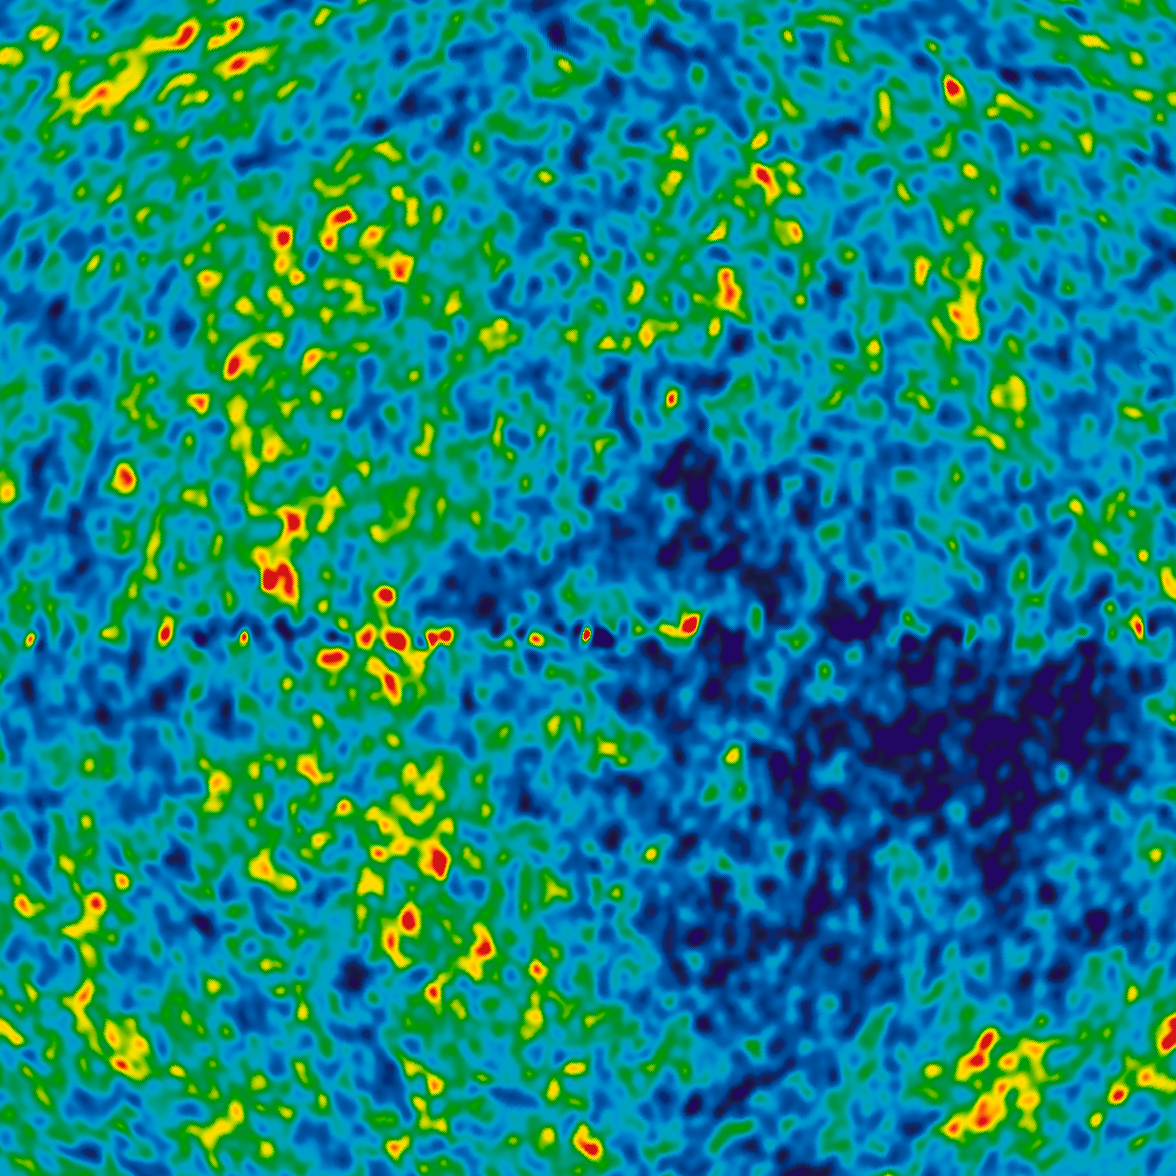
\includegraphics[width=\linewidth]{images/reliktni-zareni.png}
    \begin{center}
        mapa~teplotního rozložení~raného~vesmíru
      \end{center}
  \endminipage\hfill
  \minipage{0.3\textwidth}
    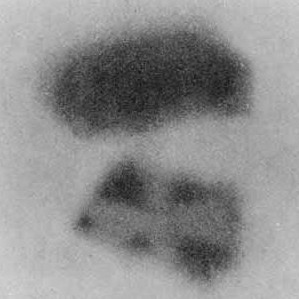
\includegraphics[width=\linewidth]{images/becquerel.jpg}
    \begin{center}
        interakce~radioaktivního záření~s~fotografickou deskou
      \end{center}
  \endminipage\hfill
  \minipage{0.3\textwidth}%
    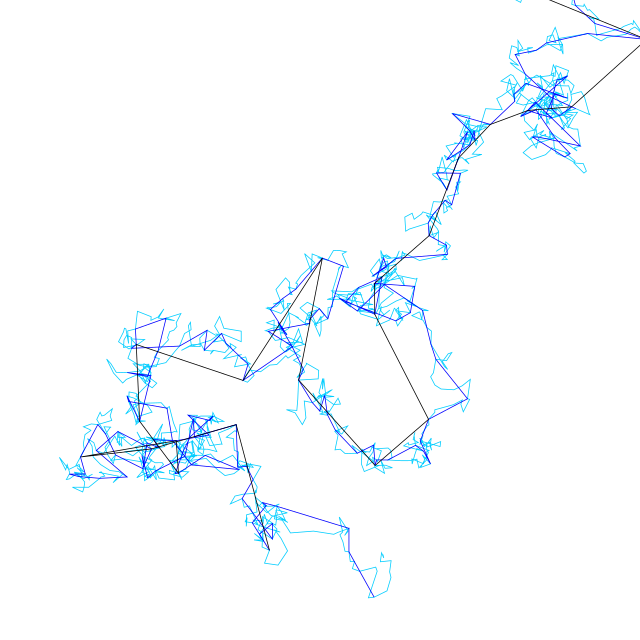
\includegraphics[width=\linewidth]{images/brownuv-pohyb.png}
    \begin{center}
        simulace~brownova pohybu~částice
    \end{center}
  \endminipage
\end{figure}
\vspace{0.5cm}
\begin{figure}[H]
  \minipage{0.3\textwidth}
    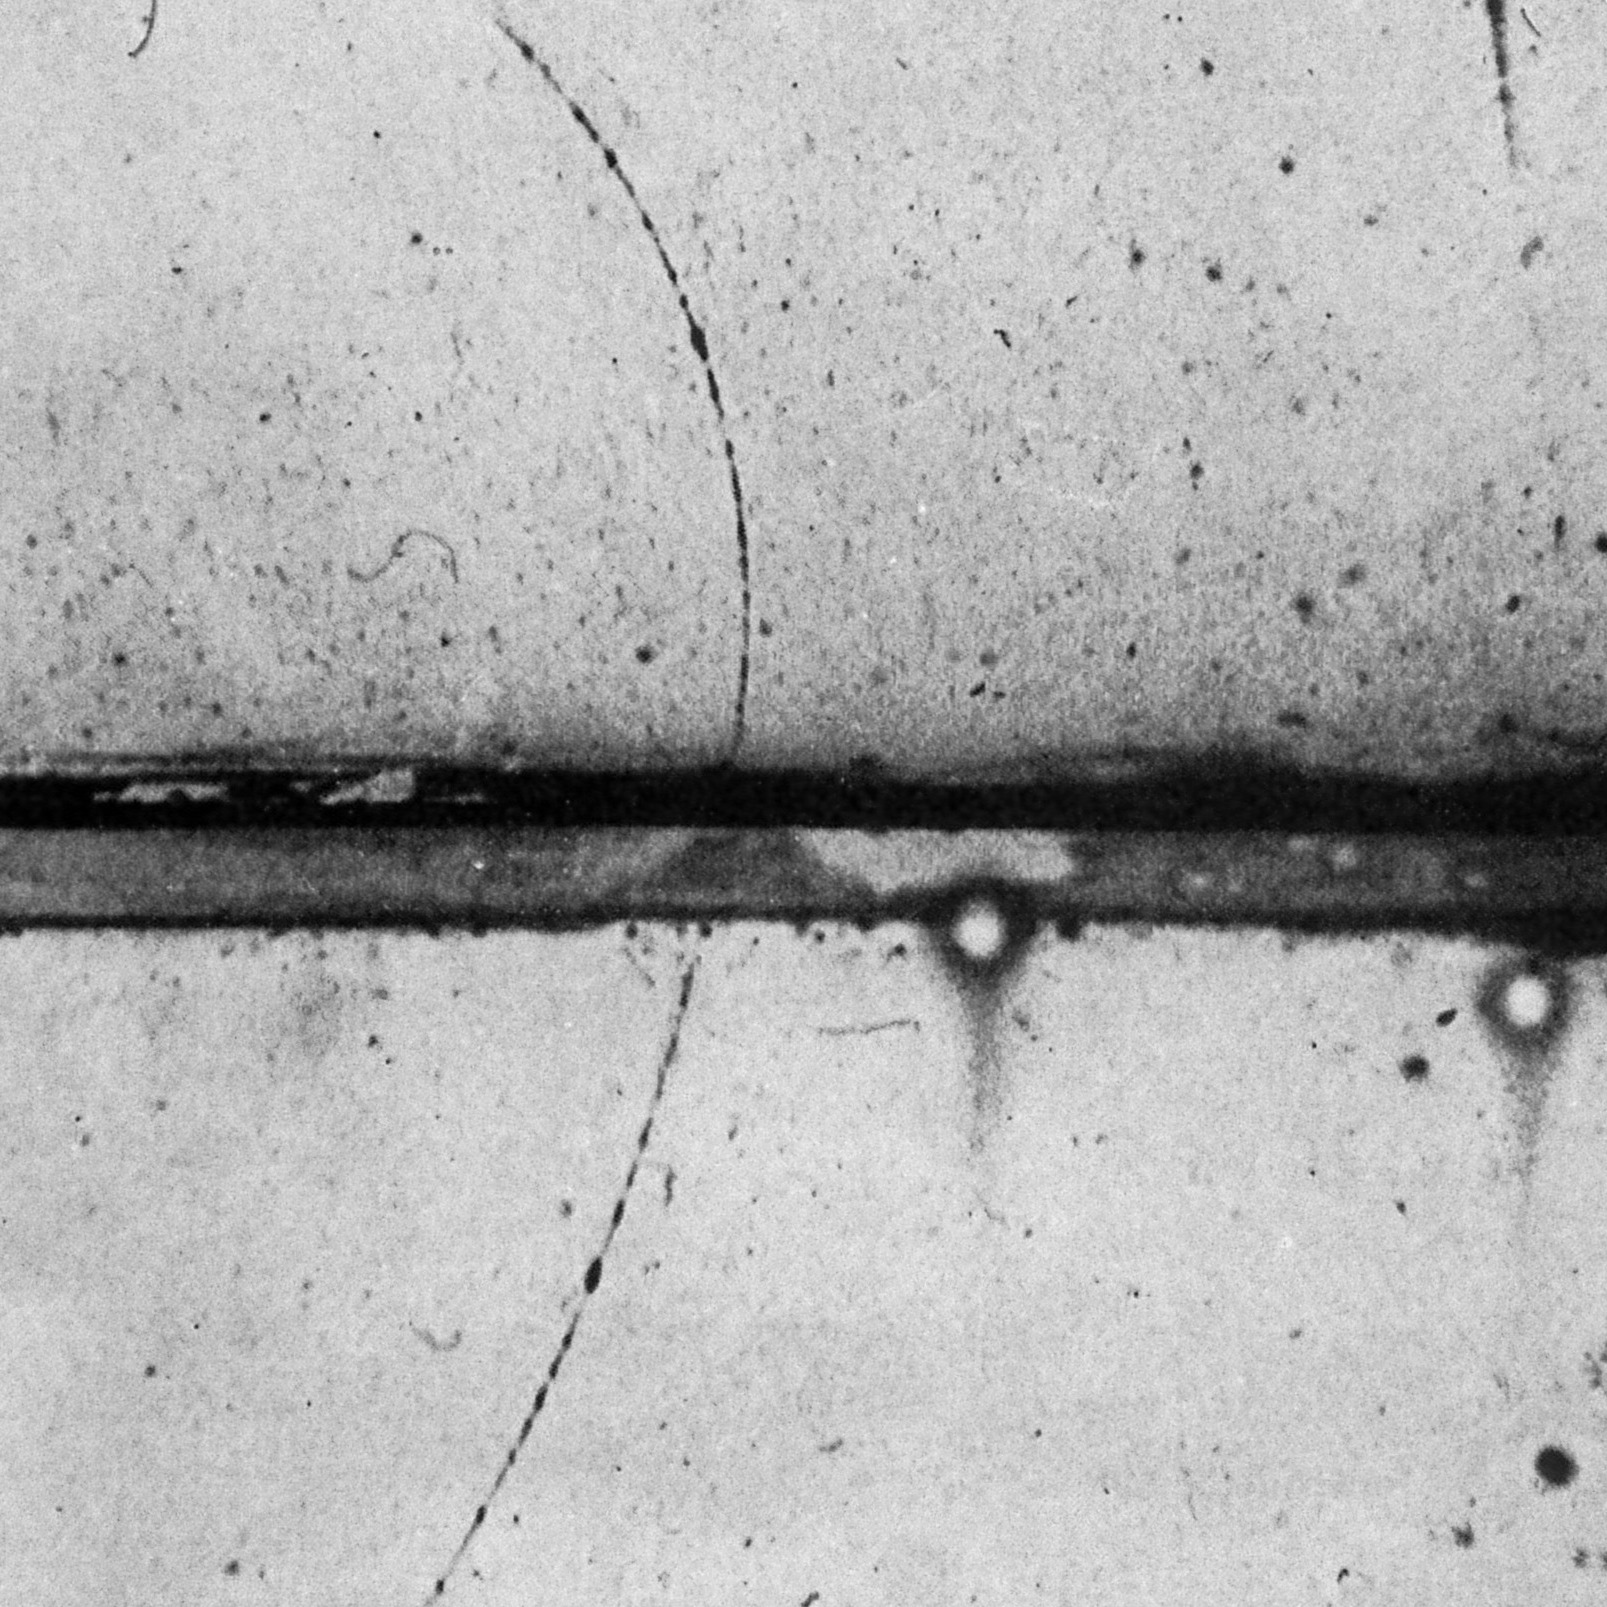
\includegraphics[width=\linewidth]{images/pozitron.jpg}
    \begin{center}
        elektron~letící~zpátky~v čase~mlžnou~komorou
      \end{center}
  \endminipage\hfill
  \minipage{0.3\textwidth}
    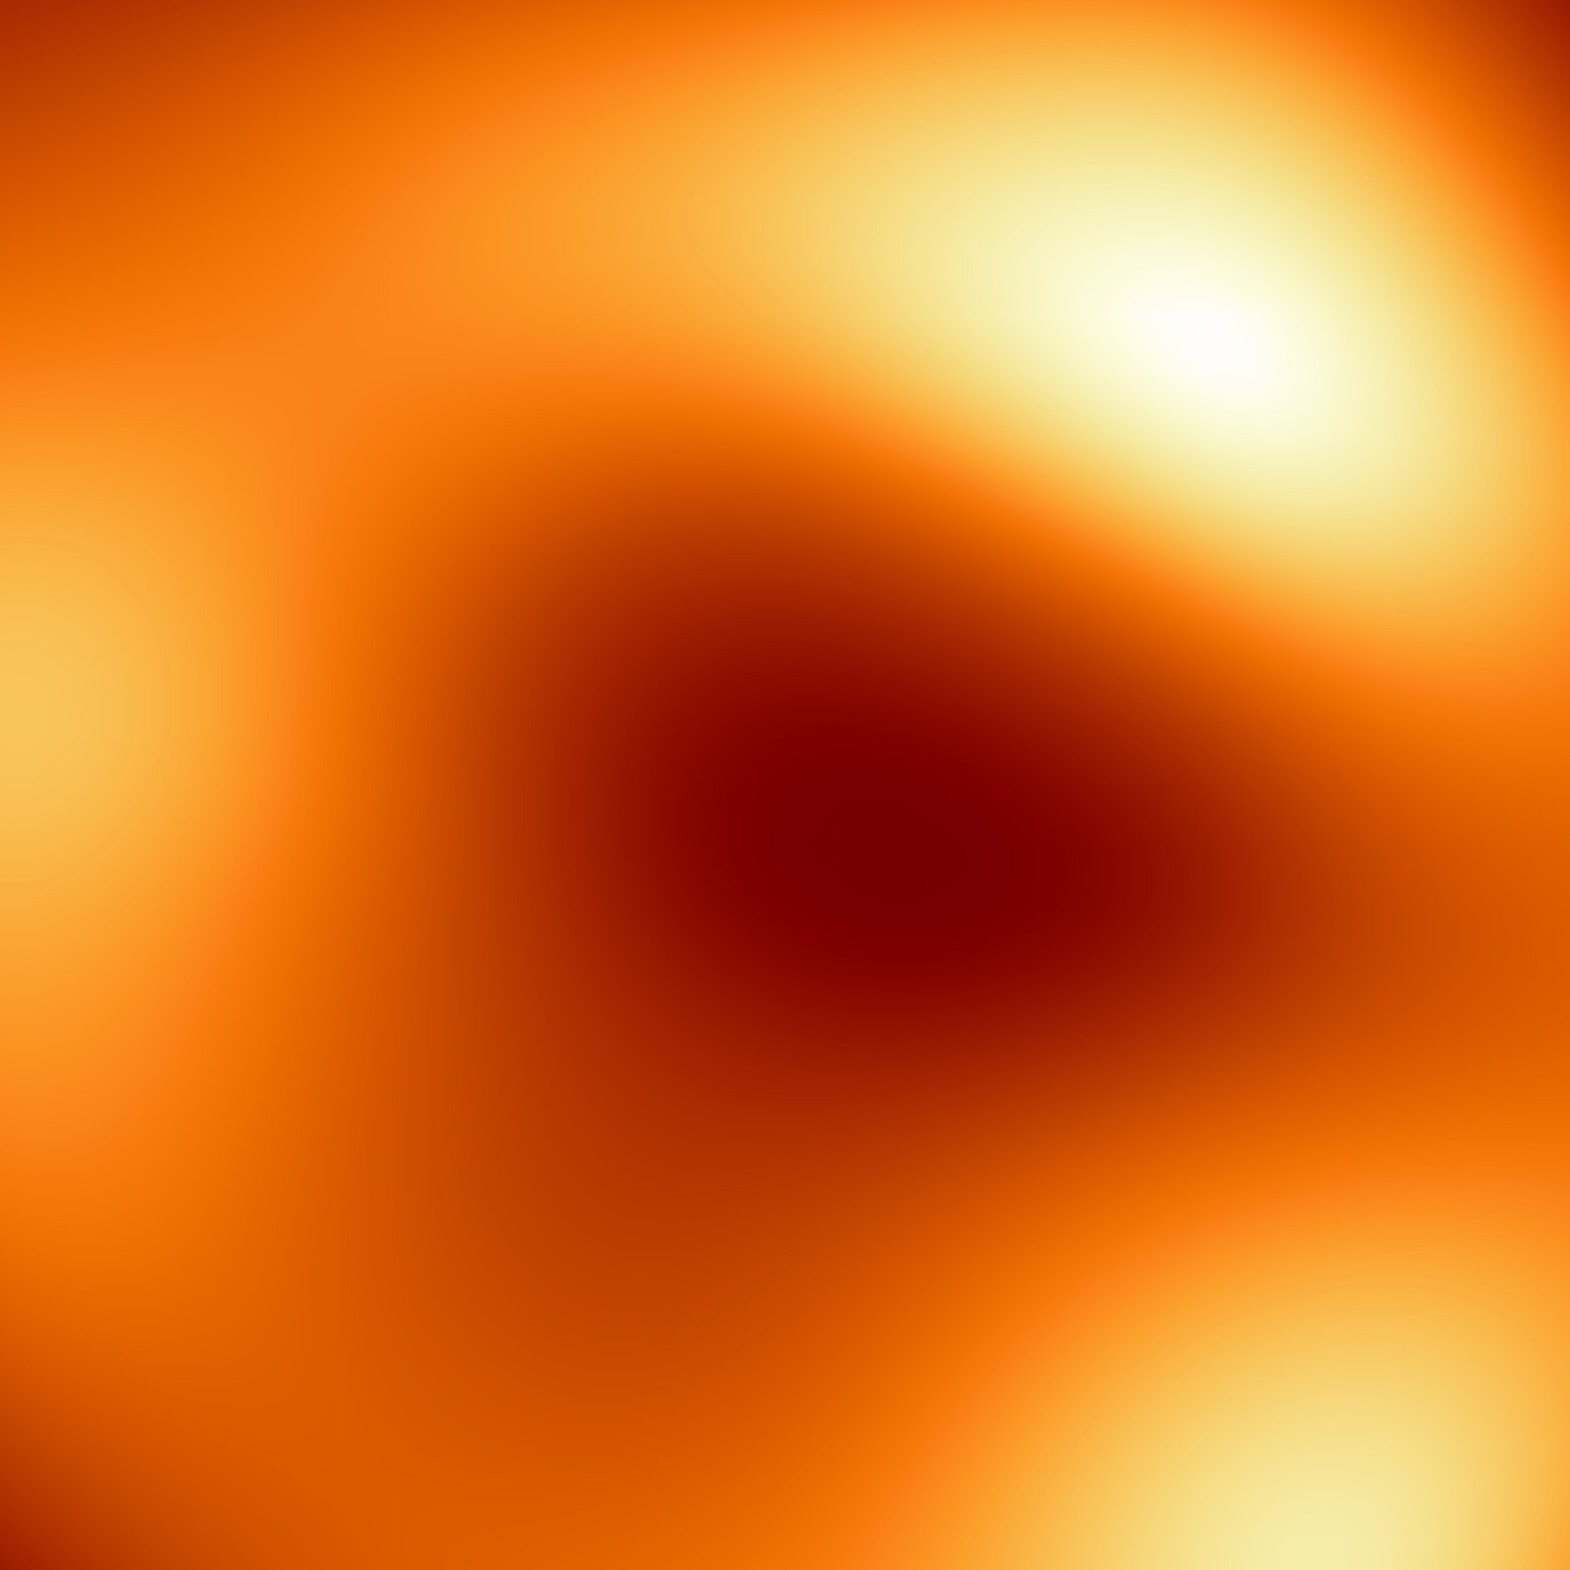
\includegraphics[width=\linewidth]{images/sagittarius.jpg}
    \begin{center}
        Sgr~A*\\\ \\
      \end{center}
  \endminipage\hfill
  \minipage{0.3\textwidth}%
    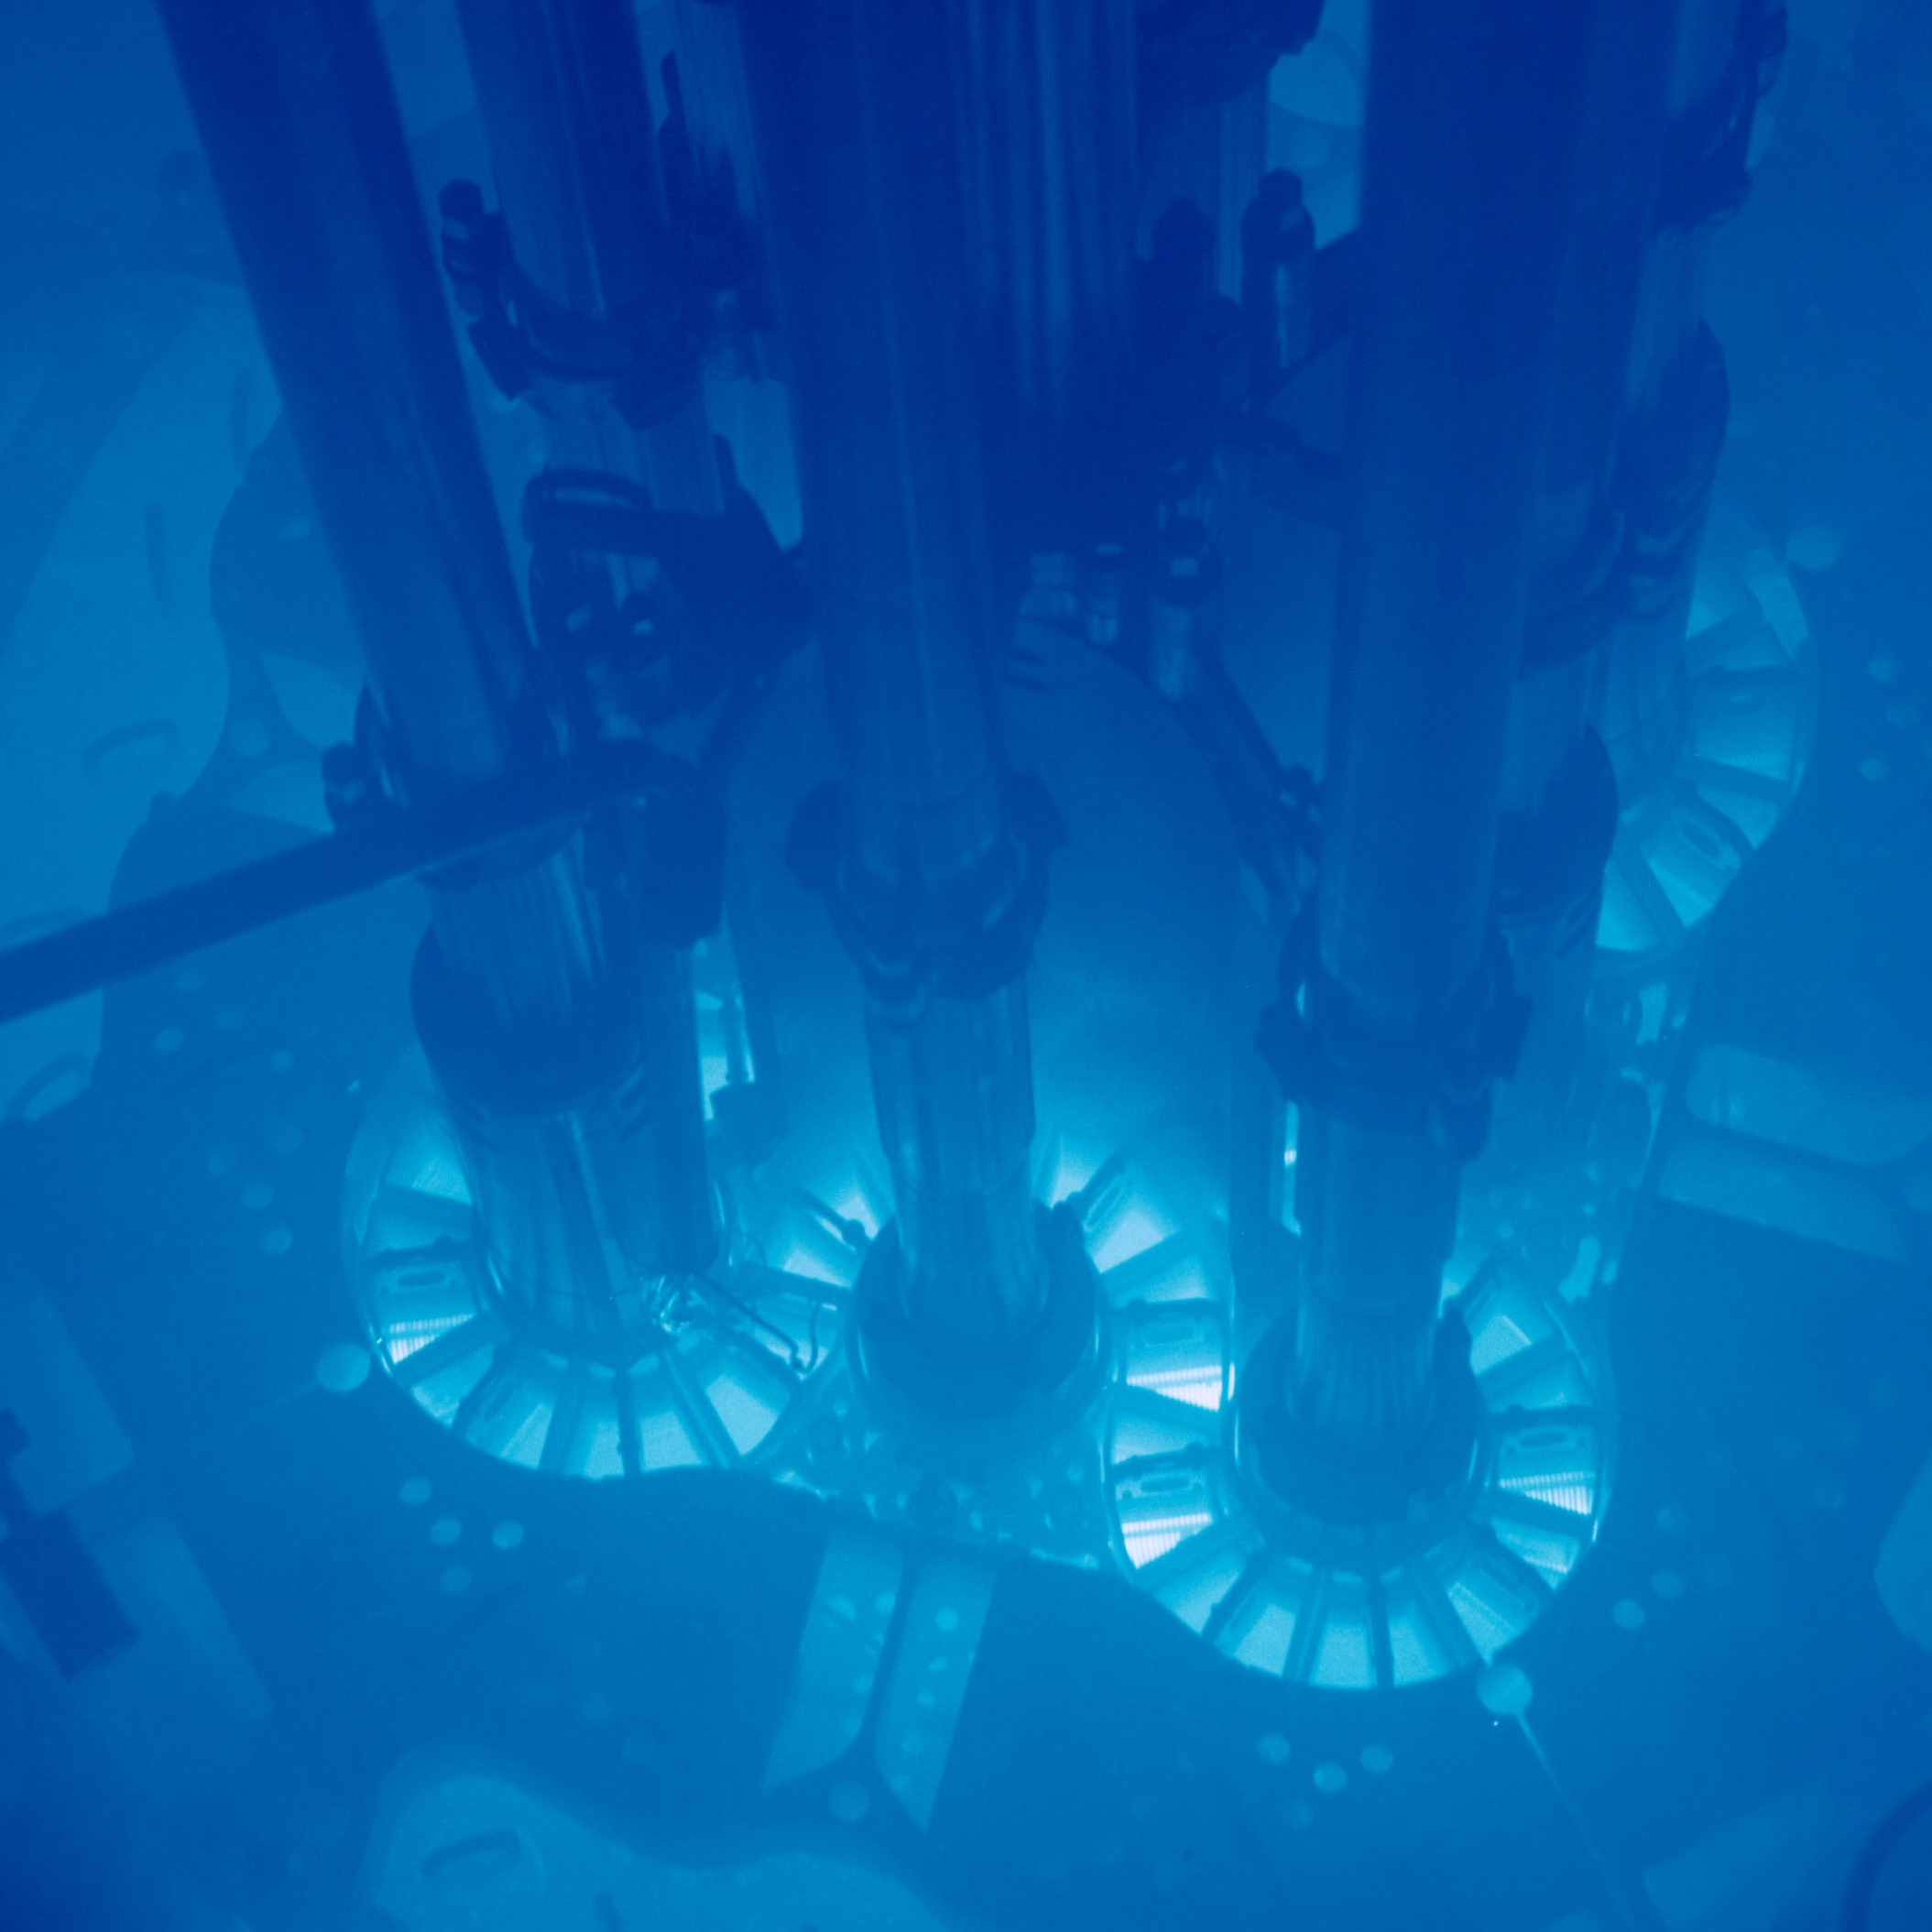
\includegraphics[width=\linewidth]{images/zareni.jpg}
    \begin{center}
        čerenkovovo~záření\\\ \\
      \end{center}
  \endminipage
\end{figure}
\noindent\textbf{Bonus:}
Jak jinak byste mohli pojmenovat 4. obrázek?

\footnotetext[1]{Autor: NASA/WMAP Science Team}
\footnotetext[2]{Autor: Henri Becquerel}
\footnotetext[3]{Autor: Di Gama}
\footnotetext[4]{Autor: Carl D. Anderson}
\footnotetext[5]{Autor: EHT Collaboration}
\footnotetext[6]{Autor: Argonne National Laboratory}
\end{document}
